% !TeX spellcheck = en_US
% !TeX program = xelatex
% !TeX root = ../md2-user-handbook.tex

\subsection{Developing a Single App} 
\label{subsec:SingleAppDev}
In this section it is described how an application can be developed based on the current (March 2015) state of the MD2 DSL. To this end, this section is structured according to the different layers which constitute \MD model and are represented in Figure \ref{fig:MD2Arch}. Aside from the conventional MVC layers -- model, view and controller -- this includes an additional layer, which enables and models the generation of workflows within and across apps and was established during the project seminar.

\begin{figure}[htb!]
\centering
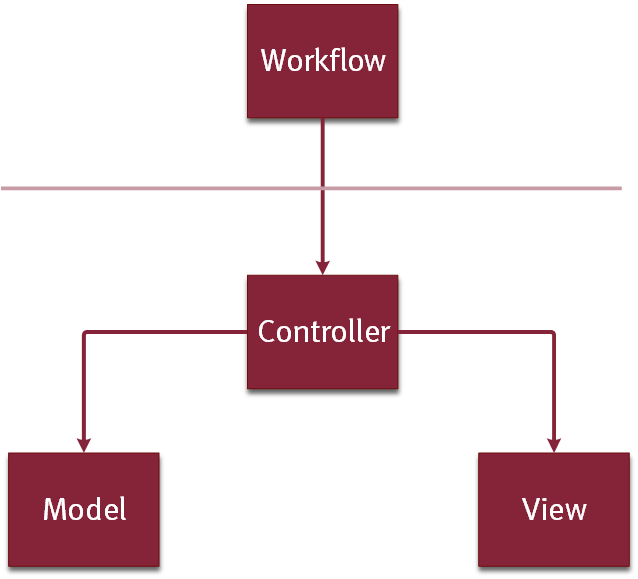
\includegraphics[width = 0.4\linewidth]{Fig/MD2Arch.png}
\caption{Architecture of \MD Models}
\label{fig:MD2Arch}
\end{figure}

All components in \MD are organized in a package structure that represents the aforementioned structure. All documents have to be placed in corresponding packages (views, models, controllers or workflow). For example, all view files are expected to be in the package any.project.package.views. The package has to be defined in each \MD file as follows:
\begin{lstlisting}
package PACKAGE_NAME
\end{lstlisting}
The package name has to be a fully qualified name that reflects the actual folder structure.

\subsubsection{Workflow} 
\label{subsubsec:Workflow}
The workflow layer is an additional abstraction on top of the controller layer. It thereby allows to specify the general course of action of one or more apps with few simple and well understandable model language constructs. Furthermore, this abstract workflow representation is intended to serve as a basis for communication with customers, e.g. for requirements engineering and collaborative app development.

In the workflow file of an MD2 model a workflow can be specified as a (possibly cyclic) directed graph of workflow elements. Workflow elements represent encapsulated functionality which is specified in detail in the controller layer. The workflow layer references the workflow elements from the controller layer to define their interaction.

For this purpose, Workflow elements are linked via events. For each workflow element one or more events can be specified that can be fired. However, at runtime a workflow element can fire only one of these events, i.e. a parallel processing of the workflow is not intended. In addition to the events that can be fired, the workflow element also specifies which workflow element is to be started in response to a fired event using the keyword {\lstinline!start!}.
A workflow element in the workflow layer typically looks as shown in Listing \ref{lst:wfe}.

\begin{lstlisting}[language=MD2, label=lst:wfe, caption=Workflow Elements in the Workflow Layer]
 WorkflowElement NameOfWorkflowElement
 	fires NameOfEventOne {
		start NameOfSubsequentWfeOne
	}
	fires NameOfEventTwo {
		start NameOfSubsequentWfe
	}
\end{lstlisting}

After defining the sequence of workflow elements, the workflow also requires the specification of an app. As shown in Listing \ref{lst:app}, an app consists of its ID, a list of workflow elements that are used in the app and a name that is to be used as app titel. For the scenario where only a single app is modeled, all workflow elements can be listed in the app. However, it is also possible to have unused workflow elements.

\begin{lstlisting}[language=MD2, label=lst:app, caption=App Definition in MD2]
App AppID {
	WorkflowElements {
		WorkflowElementOne,
		WorkflowElementTwo (startable: "Start Workflow Element Two"),
		WorkflowElementThree 
	}
	appName "App Title"
}
\end{lstlisting}

A workflow has one or more entry points, i.e. startable workflow elements. These are marked as {\lstinline!startable!} in the app specification. During code generation this will result in a button within the app that starts the corresponding workflow element. In addition, a string needs to be inserted which is used as label or description for the button.

Finally, the complete workflow specification for one app will be structured as shown in Listing \ref{lst:workflow}. Note that MD2 does not differentiate between different workflows. However, it is possible to implicitly create multiple workflows by using two or more startable workflow elements that start independent, disjunct sequences of workflow elements.

\begin{lstlisting}[language=MD2, label=lst:workflow, caption=Workflow Definition in MD2]
package ProjectName.workflows

WorkflowElement WorkflowElementOne
[...]
WorkflowElement WorkflowElementTwo
[...]
WorkflowElement WorkflowElementThree
[...]

App AppID {
	[...]
}
\end{lstlisting}

\subsubsection{Model} 
\label{subsubsec:Model}

In the model layer the structure of data objects is being described. As model elements Entities and Enums are supported.
\paragraph{Entity}
An entity is indicated by the keyword {\lstinline!entity!} followed by an arbitrary name that identifies it.
\begin{lstlisting}
entity NAME {
<attribute1 ... attribute n>
}
\end{lstlisting}
Each entity may contain an arbitrary number of attributes of the form
\begin{lstlisting}
ATTRIBUTE_NAME: <datatype>[] (<parameters>) {
name STRING
description STRING
}
\end{lstlisting}
The optional square brackets [] indicate a one-to-many relationship. That means that the corresponding object may hold an arbitrary number of values of the given datatype.
Supported complex data types are:
\begin{itemize}
\item{Entity}
\item{Enum}
\end{itemize}
Supported simple data types are:

\begin{itemize}
\item{\lstinline!integer! -- integer}
\item{\lstinline!float! -- float of the form \#.\#}
\item{\lstinline!boolean! -- boolean}
\item{\lstinline!string! -- a string that is embraced by single quotes (') or double quotes (")}
\item{\lstinline!date! -- a date is a string that conforms the following format: \lstinline!YYYY-MM-DD!}
\item{\lstinline!time! -- a time is a string that conforms the following format: \lstinline!hh:mm:ss[(+|-)hh[:mm]]!}
\item{\lstinline!datetime! -- a date time is a string that conforms the following format: \lstinline!YYYY-MM-DDThh:mm:ss [(+|-)hh[:mm]]!}
\end{itemize}

Parameters are optional and will be transformed into implicit validators during the generation process. They have to be specified as a comma-separated list. On default each specified attribute is mandatory. To allow null values the parameter optional can be set. Further supported parameters depend on the used data type and are explained as follows:

\begin{itemize}
\item \lstinline!integer! supports
\subitem \lstinline!max INTEGER! – maximum allowed value of the attribute
\subitem \lstinline!min INTEGER! – minimum allowed value of the attribute
\item \lstinline!float! supports
\subitem \lstinline!max FLOAT! – maximum allowed value of the attribute
\subitem \lstinline!min FLOAT! – minimum allowed value of the attribute
\item \lstinline!string! supports
\subitem \lstinline!maxLength INTEGER! – maximal length of the string value
\subitem \lstinline!minLingth INTEGER! – minimal length of the string value
\end{itemize}

Optionally, attributes can be annotated with a name and a description which are used for the labels and the tooltips in the auto-generation of views. If a tooltip is annotated a question mark will be shown next to the generated input field. If no name is annotated, a standard text for the label will be derived from the attribute's name by transforming the camel case name to natural language. E.g. the implicit label text of the attribute firstName is \enquote{First name}.

Exemplary entity that represents a person:
\begin{lstlisting}
entity Person {
	name: string
	birthdate: date {
		name: "Date of Birth"
		description: "The exact day of birth of this person."
	}
	salary: float (optional, min 8.50, max 1000)
	addresses: Address[]
}
\end{lstlisting}

\paragraph{Enum}
An enumeration is indicated by the keyword \lstinline!enum! followed by an arbitrary name that identifies it. Each enum may contain an arbitrary number of comma-separated strings. Other data types are not supported.
Exemplary enum element to specify weekdays:
\begin{lstlisting}
enum Weekday {
"Mon", "Tue", "Wed", "Thu", "Fri", "Sat", "Sun"
}
\end{lstlisting}


\subsubsection{View} 
\label{subsubsec:View}

\subsubsection{Controller} 
\label{subsubsec:Controller}


\subsection{Deploying a Single App}
\label{subsec:SingleAppDep}

\subsubsection{Backend} 
\label{subsubsec:Backend}

\subsubsection{map.apps} 
\label{subsubsec:mapapps}
